\documentclass{article}
\usepackage{v-test-paper}

\title{\textsc{Coordinate System}}

\begin{document}
\maketitle

\begin{itemize}
    \item Location of a point on a line
    \begin{quote}
        \textit{
            Imagine a world where you can only move in two directions: forward and backward. You can't move left or right, up or down—only along a single straight path. This path is called the x-axis. The x-axis is a horizontal line that extends infinitely in both directions. \\[2mm]
            In this one-dimensional world, we can describe the location of any point using a single number, which we call the coordinate of that point. This number tells us exactly how far along the x-axis the point is from a specific reference point known as the origin. The origin is the center point of the x-axis and has a coordinate of $0$.\\[2mm]
            If a point has a positive coordinate, it means the point is to the right of the origin. If a point has a negative coordinate, it means the point is to the left of the origin. The greater the number, the further the point is from the origin.
        }
    \end{quote}

        \begin{center}
            \begin{tikzpicture}
                \tzaxes(-5, 0)(5, 0.15){$x$}{}
                \tzticks{-4/$-4$, -3/$-3$, -2/$-2$, -1/$-1$, 0/$0$, 1/$1$, 2/$2$, 3/$3$, 4/$4$}{}
                \tzticks*{-4, -3, -2, -1, 1, 2, 3, 4}{}
            \end{tikzpicture}
        \end{center}

    \item Location of a point in a plane
    \begin{quote}
        \textit{
            Imagine a world where you can move not just forward and backward, but also left and right. This world is two-dimensional, meaning it has two directions or axes along which you can move: the x-axis and the y-axis.\\[2mm]
            The x-axis is a horizontal line that runs from left to right, and the y-axis is a vertical line that runs from bottom to top. These two lines intersect at a point called the origin, which has the coordinates (0, 0).
            In this two-dimensional world, we can describe the location of any point using a pair of numbers called coordinates. These coordinates are written as (x, y):\\[2mm]
            The first number, x, tells us how far along the x-axis the point is from the origin. A positive x value means the point is to the right of the origin, while a negative x value means the point is to the left.
            The second number, y, tells us how far along the y-axis the point is from the origin. A positive y value means the point is above the origin, while a negative y value means the point is below.
        }
    \end{quote}

        \begin{center}
            \begin{tikzpicture}
                \tzaxes(-5, -4)(5, 4){$x$}{$y$}
            \end{tikzpicture}
        \end{center}

\end{itemize}
\end{document}